
\label{subsec:ANN:SNN}

Up to now, we can talk about three generations of ANNs.
The first one comprises neurons with Boolean outputs computed by thresholded activation functions such as the hard limit function. 
The second one includes neurons suitable for analog in- and output because of continuous activation functions like sigmoid or hyperbolic tangent functions.
Spiking neurons are considered the third generation of ANNs and raise the level of biological realism of ANNs: they are capable of producing a kind of action potentials as real neurons do, allowing incorporating spatial-temporal information in the communication and computation process of ANNs, as biological neural networks do \cite{vreeken2002spiking}.

The more remarkable difference between SNN and the two first generations of ANNs is that 
the input and output of the former are not signal values as in the latter,
but the time reference of its spikes.
As we described in \subsecref{actionpotential} when talking about the spikes produced by biological neurons, 
the action potentials are very similar to each other, 
so we can forget temporally about form and characterise them by their firing times; \ie, the time between consecutive spikes each neuron produces. Thus, the $f$-th spike of neuron $j$ can be referred as $t_{j}^{(f)}$ and the complete spike-train of the same neuron as: 
\begin{equation}
\mathcal{F}_{j}=\{t^{(1)},t^{(2)}...,t^{(n)}\}
\label{eq:spiketrain}
\end{equation}

where $\mathcal{F}_{j}$ is chronologically ordered; \ie,
if $1\leq f<g \leq n$, then $t_{j}^{(f)} < t_{j}^{(g)}$.

The same way it occurs in action potentials, no spike will be fired unless the membrane potential value increases up to a critical value $\vartheta$. Denoting as $u_{j}(t)$ the membrane potential or internal state of the neuron $j$, this threshold condition can be expressed as:
\begin{equation}
\mathcal{F}_{j}=\{t\mid u_{j}(t)=\vartheta\wedge u_{j}'(t)>0\}
\label{eq:thresspikecondition}
\end{equation}

It is at this point that the neuron model of \subsecref{neuronmodel} must be revised. 
The new model has to include the spike time information in such a way as the behaviour of the membrane potential in \eref{thresspikecondition} can be implemented. 
Along these lines, there are many models of spiking neurons. Some of the most common are:
the spike response model \cite{gerstner2002spiking}, the integrate-and-fire derived from the Hodgkin-Huxley model \cite{chiu1979quantitative} and the Izhikevich's neuron model \cite{izhikevich2003simple}.
Since we have implemented the former, it is described in the following section. A brief description of the remaining models and some others can be found in \cite{paugam2012computing}.







\subsubsection{Spike Response Model}
\label{subsubsec:SRM}

The Spike Response Model (SRM) is a phenomenological model of a neuron which describes how the incoming spike-trains are processed to produce a new spike-train leaving the neuron.
For this purpose, the potential of a spiking neuron is modeled by a dynamic variable and works as a leaky integrator of the incoming spikes
so that newer spikes contribute more to the potential than
older spikes. 
Then, if this sum accomplishes \eref{thresspikecondition}, 
the neuron fires a spike.

Gerstner \etal \cite{gerstner2002spiking} describe the neuronal dynamics of the SRM through \figref{srmdynamic}. 
Centering the attention in the time course of $u_{j}(t)$, which referres to the membrane potential of neuron $j$, the following lines explain the mathematics behind the process shown in the lastmentioned figure. Notice the unavoidable similarity with the behaviour of the biological neurons described in \subsecref{actionpotential}.

\begin{description}

\item {\textbf{\figref{srmdynamic} A}\hfill \\
Before any input has arrived, neuron $j$ is in the resting state, so $u_{j}(t)=u_{\text{rest}}$.
If a presynaptic neuron $i=1$ fired at $t_{i}^{(f)} \in \mathcal{F}_{i}$, we see at the electrode a response of neuron $j$ that can be expressed as
\begin{equation}
u_{j}(t-t_{i}^{(f)})-u_{\text{rest}}=\varepsilon(t-t_{i}^{(f)})
\label{eq:postsynapticpotential}
\end{equation}
where $\varepsilon$, called \emph{spike response function}
or \emph{postsynaptic potential} (PSP), 
emulates the contribution of one synaptic terminal on the potential of the postsynaptic neuron caused by a presynaptic spike.
}

\item {\textbf{\figref{srmdynamic} B}\hfill \\
If another input spike (for example from a presynaptic neuron $i=2$) arrives after the previous spike, a new PSP will be evoked and its effect will be added to that of the first spike. Extending the concept to multiple spikes from several neurons, this process can be denoted as
\begin{equation}
u_{j}(t)=\sum_{i\in \Gamma_{j}}\sum_{f\in \mathcal{F}_{i}}
	\varepsilon(t-t_{i}^{(f)})+u_{\text{rest}}
\label{eq:pspgeneralised}
\end{equation}
where $\Gamma_{j}$ referres to the set of presynaptics neurons $i$ of the postsynaptic one $j$. Then, $f$ is the $f$-th spike of the spike-train $\mathcal{F}_{i}$ that each presynaptic neuron $i$ fires. This way, in the SRM, the membrane potential responds linearly to input spikes.
}

\item {\textbf{\figref{srmdynamic} C}\hfill \\
The aforesaid linearity breaks down if the amount of spikes arrived during a short interval makes the membrane potential $u_{j}$ reach the critical value $\vartheta$. In that situation, \eref{thresspikecondition} is accomplished and an action potential is triggered. The membrane potential sufferes then a peak of pulse (out of bounds in \figref{srmdynamic}C) and then returns to the resting potential after passing through a phase of hyperpolarization below the resting value. This 
%negative overshoot 
process is modeled with a certain standard time course denoted by $\eta(t-t_{j}^{(f)})$, where $t_{j}^{(f)}$ referres the firing time, which is defined by the moment of threshold $\vartheta$ crossing. Consequently, as far as the membrane potential is concerned, the spike-train of neuron $j$ can be expressed as
\begin{equation}
u_{j}(t)=\sum_{f\in \mathcal{F}_{j}}\eta(t-t_{j}^{(f)})
\label{eq:refractoriness}
\end{equation}

Therefore, $\eta$ must model the positive pulse and the negative overshoot of the action potential. Since the spikes are characterised by their firing times, the positive pulse has no real significance. In contrast, the negative part has an important application: it comprises the ``reset'' of the membrane potential. Moreover, if the negative overshoot makes the membrane potential fall far below the threshold $\vartheta$, the emission of another pulse immediately after one is then more difficult (many PSPs are needed to reach again the threshold). This way, the negative overshoot of $\eta$ models not only the ``reset'', but also the refractory period or refractoriness of the neuron.
}

\end{description}

\begin{figure}[!ht]
\centering
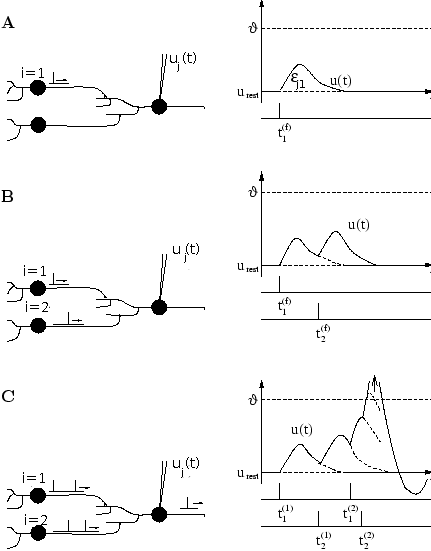
\includegraphics[width=0.8\textwidth]{images/srm_dynamics_png.png}
\caption{Postsynaptic neuron $j$ receives input from two presynaptic neurons $j=1,2$.}
\label{fig:srmdynamic}
\end{figure} 

Combinig in neuron $j$ the PSPs evoked by the spikes of its presynaptic neurons (\eref{postsynapticpotential}) and the refractoriness effect caused by its own action potential (\eref{refractoriness}), the time course of its membrane potential is modeled by
\begin{equation}
u_{j}(t)=\sum_{f\in \mathcal{F}_{j}}\eta(t-t_{j}^{(f)})+
\sum_{i\in \Gamma_{j}}\sum_{f\in \mathcal{F}_{i}}
	\varepsilon(t-t_{i}^{(f)})+u_{\text{rest}}
\label{eq:srmuniqueconnection}
\end{equation}


As it occurs with the other ANNs topologies described in this chapter,
the strength of the synapse involving the presynaptic neuron $i$ and the postsynaptic neuron $j$ is modeled with a weight term $w_{ji}$.
Furthermore, in order to incorporate spatial-temporal information in the communication, SNNs include the axonal delay $d_{ji}$ caused by the signal transmission from the soma of neuron $i$ to the dendrites of neuron $j$.

Now, if we imagine a neural network like the one shown in \figref{snn}, 
where every connection consists of $1 \leq k \leq m$ synapses with different weights and delays, 
the resultant SRM of the spiking neuron $j$ can be expressed as

\begin{equation}
u_{j}(t)=
\sum_{f\in \mathcal{F}_{j}}\eta(t-t_{j}^{(f)})+
\sum_{i\in \Gamma_{j}}
\sum_{f\in \mathcal{F}_{i}}
\sum_{k=1}^{m}
	w_{ji}^{k}\varepsilon(t-t_{i}^{(f)}-d_{ji}^k)+u_{\text{rest}}
\label{eq:srmmultipleconnections}
\end{equation}

where $w_{ji}^k$ and $d_{ji}^k$ refer the weight and delay of the connection $k$ from the presynaptic neuron $i$ to the postsynaptic one $j$ respectively.

\begin{figure}[!ht]
\centering
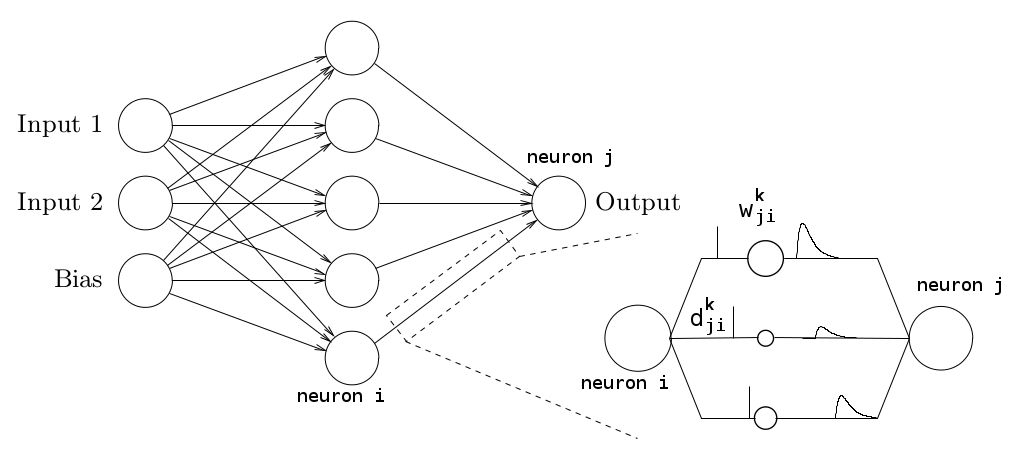
\includegraphics[width=1\textwidth]{images/snn.png}
\caption{Spiking neural network model}
\label{fig:snn}
\end{figure} 

Finally, it is important to notice that, in \etoref{postsynapticpotential}{srmmultipleconnections} we are considering the resting potential term. However, since only the potential difference -the distance from the resting potential- is relevant, we can always set $u_{\text{rest}}=0$ by applying an appropriate linear shift of scale.